% !TEX encoding = UTF-8 Unicode

\documentclass[a4paper]{article}

\usepackage{color}
\usepackage{url}
\usepackage[utf8]{inputenc}
\usepackage{graphicx}
\usepackage[english,serbian]{babel}
\usepackage[unicode]{hyperref}
\usepackage{amsmath}
\usepackage{amsthm}
\usepackage{amssymb}
\hypersetup{colorlinks,citecolor=green,filecolor=green,linkcolor=blue,urlcolor=blue}
\usepackage[title]{appendix}
\usepackage{float}
\usepackage[graphicx]{realboxes}
\usepackage[font=small,labelfont=bf]{caption}
\usepackage{chngcntr}
\counterwithin{figure}{section}
\usepackage{listings}
\usepackage{textcomp}
\usepackage{xcolor}
\lstset {
    language=C++,
    frame=single,
    framesep=10pt,
    tabsize=4,
    showstringspaces=false,
    upquote=true,
    commentstyle=\color{commentgreen},
    keywordstyle=\color{orange},
    stringstyle=\color{red},
    basicstyle=\small\ttfamily,
    emph={int,char,double,float,unsigned,void,bool},
    emphstyle={\color{blue}},
    escapechar=\&,
    % keyword highlighting
    classoffset=1, % starting new class
    morekeywords={>,<,.,;,,,-,!,=,~},
    keywordstyle=\color{weborange},
    classoffset=0,
}

\theoremstyle{plain}
\newtheorem{thm}{Teorema}[section]
\theoremstyle{definition}
\newtheorem{defn}[thm]{Definicija}
\newtheorem{exmp}[thm]{Primer}
\newtheorem{assn}[thm]{Pretpostavka}
\newtheorem{obsn}[thm]{Zapa\v{z}anje}


\begin{document}

\title{Binarni dijagrami odlu\v{c}ivanja\\ \small{Seminarski rad u okviru kursa\\Automatsko rezonovanje\\ Matematički fakultet}}

\author{\href{mailto:mi14031@matf.bg.ac.rs}{Milana Kova\v{c}evi\'c}\\\href{mailto:mi14042@matf.bg.ac.rs}{Ivan Ristovi\'c}}
\date{jul 2018.}

\maketitle

\emph{Binarni dijagrami odlu\v{c}ivanja} (u daljem tekstu \emph{BDD}) i njihova pobolj\v{s}anja su strukture podataka za reprezentaciju bulovskih funkcija. Iako u osnovi sli\v{c}ni binarnim drvetima, re\v{s}avaju problem velikog broja \v{c}vorova u drvetu uklanjaju\'c{}i redundantne grane (za bulovsku funkciju sa $n$ argumenata, broj mogu\'c{}ih puteva u binarnom drvetu od korena do lista je $2^{n}$, dok je broj \v{c}vorova znatno ve\'c{}i). U ovom radu \'c{}emo detaljnije opisati ideju na kojoj su zasnovani BDD, na\v{c}ine za njihovu konstrukciju, kao i razne varijante BDD - \emph{ROBDD}, \emph{FBDD} i \emph{ZDD}. Ovaj rad \'c{}e pratiti implementacija ROBDD u jeziku \emph{C++}, uz prate\'c{}e delove koda na nekim mestima.


\tableofcontents

\newpage

\section{Bulovske funkcije}
\label{sec:BulovskeFunkcije}

\emph{Bulovske funkcije} su funkcije koje primaju argumente koji su bulovske vrednosti i vra\'c{}aju bulovsku vrednost. Bulovske vrednosti mogu biti \emph{true} ili \emph{false}. U nastavku \'c{}emo sa $1$ ozna\v{c}avati \emph{true}, a sa $0$ \emph{false}, \v{s}to je uobi\v{c}ajena konvencija.

Za bulovsku funkciju sa $n$ bulovskih argumenata, postoji $2^{n}$ mogu\'c{}ih ulaza. Po\v{s}to je povratna vrednost takodje bulovskog tipa, zaklju\v{c}ujemo da postoji $2^{2^{n}}$ razli\v{c}itih bulovskih funkcija sa $n$ argumenata, \v{s}to se vidi iz jednakosti

\[ \underbrace{2*2*2* \dotsb *2}_{\text{$2^{n}$}} = 2^{2^{n}} \]

Funkcije koje primaju neozna\v{c}eni broj u opsegu $[0,2^{n}-1]$ se mogu zameniti sa $n$ bulovskih funkcija sa $n$ argumenata. Kao primer, neka je data funkcija $F$ koja prima i vra\'c{}a neozna\v{c}eni ceo broj. Zamenjujemo funkciju $F$ bulovskim funkcijama $f_i$, $i = 0, 1, \dots , n-1$. Argumenti funkcije $f_{i}$ su $n$ binarnih cifara broja, dok je povratna vrednost $f_{i}$ vrednost $i$-te binarne cifre rezultata funkcije $F$. Drugim re\v{c}ima, svaka od funkcija $f_{i}$ ra\v{c}una jednu cifru rezultata. Kao konkretan primer, s obzirom da su neozna\v{c}eni brojevi u ra\v{c}unarima zauzimaju obi\v{c}no $32$ bita, funkciju

\begin{lstlisting}[language=C++]
    unsigned F(unsigned n);
\end{lstlisting}

\noindent mo\v{z}emo zameniti sa $32$ bulovske funkcije

\begin{lstlisting}[language=C, emph={bool}]
    bool f0(bool n0, bool n1, bool n2, ... , bool n31);
    bool f1(bool n0, bool n1, bool n2, ... , bool n31);
    ...
    bool f31(bool n0, bool n1, bool n2, ... , bool n31);
\end{lstlisting}

Naravno, moramo se uveriti da su cifre rezultata zaista jednake izlazima bulovskih funkcija. Jedan na\v{c}in za verifikaciju rezultata je primena obe tehnike nad svim mogu\'c{}im ulazima i poredjenje dobijenih rezultata. Medjutim, \v{c}ak i za ovako jednostavne funkcije re\v{c} je o oko 4 milijarde ($2^{32}$) mogu\'c{}ih ulaza. Drugi na\v{c}in je da se ove funkcije prika\v{z}u putem nekih struktura podataka, i da se funkcije porede tako \v{s}to se porede njihove reprezentacije preko tih struktura. Drugim re\v{c}ima, posmatramo funkcije kao podatke. U poglavljima koji slede \'c{}e biti vi\v{s}e re\v{c}i o strukturama podataka koje se koriste za predstavljanje bulovskih funkcija. Takodje, u narednim poglavljima pod terminom \emph{funkcija} \'c{}emo podrazumevati bulovske funkcije, ukoliko to nije druga\v{c}ije nazna\v{c}eno.

\section{Binarna drveta odlu\v{c}ivanja}
\label{sec:BinarnaDrvetaOdlucivanja}

Binarna drveta odlu\v{c}ivanja su u osnovi jako sli\v{c}na binarnim drvetima. Na ovom nivou radimo sa bulovskim funkcijama. Neka je dato $n$ promenljivih $x_{1}, x_{2}, \dots , x_{n}$ koje predstavljaju ulaze u bulovsku funkciju $f$. U korenom \v{c}voru testiramo jednu promenljivu (bez umanjenja op\v{s}tosti, krenu\'c{}emo redom, te neka je to $x_{1}$). U zavisnosti od vrednosti te promenljive formiraju se dva pod-drveta - jedno u kome je $x_{1} = 0$ (\emph{nisko} pod-drvo), a drugo u kome je $x_{1} = 1$ (\emph{visoko} pod-drvo). U svakom pod-drvetu se rekurzivno testiraju ostale promenljive na isti na\v{c}in. Do listova se dolazi kada vi\v{s}e nema preostalih ulaznih promenljivih. Posmatraju\'c{}i jedan put od korena do lista, dobijamo valuaciju za skup $\{x_{1}, \dots , x_{n}\}$.

Uzmimo za primer funkciju:

\begin{lstlisting}[language=C++]
    bool f_and(bool x1, bool x2) { return x1 && x2; }
\end{lstlisting}

\noindent Matematički zapis ove funkcije bi bio $x_{1} \wedge x_{2}$. Binarno drvo odlu\v{c}ivanja za ovu funkciju je dat na slici \ref{diag:BDAnd}. Polaze\'c{}i od promenljive $x_{1}$, formiramo dve grane na osnovu toga da li je $x_{1} = 0$ ili $x_{1} = 1$. Od sada pa u budu\'c{}e \'c{}emo grane u kojima je vrednost $0$ crtati isprekidanom linijom, a grane u kojima je vrednost $1$ punom linijom, zarad preglednosti.

\begin{figure}[H]
    \centering
    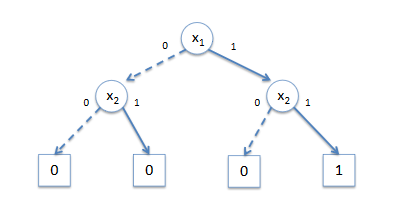
\includegraphics[scale=0.8]{slike/BD_And.PNG}
    \caption{Binarno drvo odlu\v{c}ivanja za funkciju $\wedge$}
    \label{diag:BDAnd}
\end{figure}

\noindent Sli\v{c}no se mogu definisati i ostale korisne funkcije, na primer \texttt{f\_or} ($\vee$) i \texttt{f\_xor} ($\oplus$), sa dijagramima na slici \ref{fig:BDOrXor}:

\begin{lstlisting}[language=C++,escapechar=@]
    bool f_or(bool x1, bool x2) { return x1 || x2; }

    bool f_xor(bool x1, bool x2) {
        return (x1 && !x2) || (!x1 && x2); @\footnote{Ne mo\v{z}emo koristiti operator \^{} jer on operi\v{s}e nad promenljivima tipa \emph{int}, a ne \emph{bool}.}@
    }
\end{lstlisting}

\begin{figure}[H]
    % NE DIRAJ OVE BROJEVE
    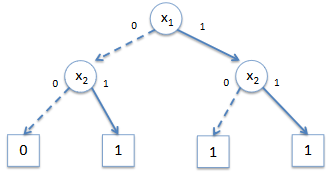
\includegraphics[scale=0.68]{slike/BD_Or.PNG}
    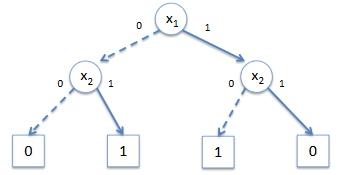
\includegraphics[scale=0.68]{slike/BD_Xor.PNG}
    \caption{Binarna drveta odlu\v{c}ivanja za funkcije $\vee$ i $\oplus$, redom}
    \label{fig:BDOrXor}
\end{figure}

Binarna drveta odlu\v{c}ivanja imaju neke veoma lo\v{s}e osobine. Najve\'c{}i problem je njihova veli\v{c}ina. Binarno drvo za $n$ ulaznih promenljivih \'c{}e imati $2^{n-1}$ unutra\v{s}njih \v{c}vorova i $2^{n}$ listova.

Uprkos tome, postoje i neke dobre osobine, pre svega \emph{kanoni\v{c}nost}. Ukoliko testiramo promenljive uvek u istom redosledu (tada se binarno drvo odlu\v{c}ivanja naziva \emph{uredjeno}), onda je drvo jedinstveno za svaku bulovsku funkciju. Stoga se test ekvivalencije dve bulovske funkcije svodi na testiranje ekvivalentnosti njivohih binarnih drveta odlu\v{c}ivanja. Na\v{z}alost, zbog velikog broja \v{c}vorova u drvetima, problem je eksponencijalne slo\v{z}enosti u odnosu na broj ulaznih parametara.

Kako bi se re\v{s}io problem eksplozije broja \v{c}vorova u drvetu, formiraju se unapredjenja binarnih drveta odlu\v{c}ivanja - binarni dijagrami odlu\v{c}ivanja (\emph{BDD}). O njima \'c{}e biti vi\v{s}e re\v{c}i u poglavlju koje sledi.

\section{Binarni dijagrami odlu\v{c}ivanja}
\label{sec:BDD}

Binarni dijagrami odlu\v{c}ivanja (engl. \emph{Binary Decision Diagrams}, u daljem tekstu \emph{BDD}) su unapredjenje binarnih drveta odlu\v{c}ivanja. Prvo unapredjenje je uklanjanje redundantnih grana u drvetu. Na primer, posmatrajmo funkciju $\wedge$ definisanu u poglavlju \ref{sec:BinarnaDrvetaOdlucivanja}. U niskom pod-drvetu obe grane koje polaze od promenljive $x_{2}$ vode ka vrednosti $0$, stoga nije potrebno ispitivati vrednost promenljive $x_{2}$ \footnote{tzv. \emph{lenjo izra\v{c}unavanje}}. Ovakvom redukcijom se dobija drvo na slici \ref{diag:BDDAnd}.

\begin{figure}[H]
    \centering
    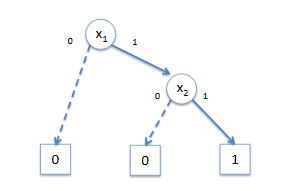
\includegraphics[scale=0.8]{slike/BDD_And.PNG}
    \caption{BDD za funkciju $\wedge$}
    \label{diag:BDDAnd}
\end{figure}

Drugo unapredjenje je dozvoljavanje deljenja identi\v{c}nih pod-drveta. Ponovo, kako bi \v{c}italac bolje razumeo \v{s}ta ovo zapravo zna\v{c}i, dajemo primer. Posmatrajmo funkciju koja ima povratnu vrednost $1$ ukoliko postoji neparan broj ulaznih promenljivih sa vredno\v{s}\'c{}u $1$, a $0$ ina\v{c}e. \v{S}tavi\v{s}e, pretpostavimo da imamo \v{c}etiri ulazne promenljive $x_{1}$, $x_{2}$, $x_{3}$ i $x_{4}$. Binarno drvo odlu\v{c}ivanja za ovakvu funkciju bi imalo 15 ($2^4 - 1$) unutra\v{s}njih \v{c}vorova i 16 ($2^4$) listova. Medjutim, BDD za ovu funkciju ima samo 7 unutra\v{s}njih \v{c}vorova i samo dva lista (slika \ref{diag:BDDParity}).

\begin{figure}[H]
    \centering
    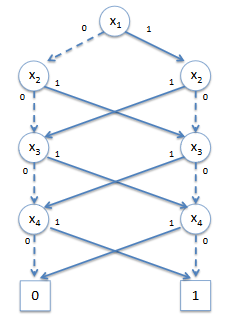
\includegraphics[scale=0.8]{slike/BDD_Parity.PNG}
    \caption{BDD za funkciju parnosti \v{c}etiri argumenta}
    \label{diag:BDDParity}
\end{figure}

U najgorem slu\v{c}aju, BDD \'c{}e biti eksponencijalno veliki u odnosu na ulaz, mada u praksi je to retko slu\v{c}aj. Takodje, konstantne funkcije se mogu predstaviti samo jednim \v{c}vorom, bez obzira na broj ulaznih promenljivih.

\section{Redukovani uredjeni binarni dijagrami odlu\v{c}ivanja (ROBDD)}
\label{sec:OBDD}

Uredjeni binarni dijagrami odlu\v{c}ivanja (engl. \emph{Ordered Binary Decision Diagrams}, u daljem tekstu \emph{OBDD}) su BDD u kojima se promenljive uvek testiraju u istom redosledu. OBDD se naziva \emph{redukovani}(engl. \emph{Reduced Ordered Binary Decision Diagrams} \cite{ROBDD}, u daljem tekstu \emph{ROBDD}) ukoliko poseduje slede\'c{}e osobine:
\begin{itemize}
    \item Neredundantnost - Visoki i niski naslednik svakog \v{c}vora je razli\v{c}it.
    \item Jedinstvenost - Ne postoje dva razli\v{c}ita \v{c}vora koja testiraju istu promenljivu, a \v{c}iji su naslednici isti.
\end{itemize}

Kao \v{s}to je pomenuto u poglavlju \ref{sec:BinarnaDrvetaOdlucivanja}, binarna drveta odlu\v{c}ivanja poseduju osobinu kanoni\v{c}nosti. Medjutim, kako postoje razli\v{c}iti BDD koja odgovaraju jednom binarnom drvetu odlu\v{c}ivanja, jasno je da BDD nemaju ovu osobinu. Uprkos tome, zbog svojih lepih i jasno definisanih osobina, ROBDD su takodje kanoni\v{c}ni. Pro\v{s}irivanjem definicije kanoni\v{c}nosti na ROBDD, dolazimo do slede\'c{}eg zapa\v{z}ivanja

\begin{obsn}
    Kanoni\v{c}nost ROBDD povla\v{c}i da za fiksni redosled promenljivih, svaka funkcija ima jedinstvenu reprezentaciju u vidu ROBDD. To zna\v{c}i da mo\v{z}emo ekvivalentnost dve funkcije testirati tako \v{s}to \'c{}emo porediti njihove ROBDD.
\end{obsn}

ROBDD ima najvi\v{s}e dva lista - 0 i 1 (\emph{konstatni listovi} ili \emph{listovi-konstante}). U nastavku \'c{}emo ponekad crtati vi\v{s}e istih listova kako bi se smanjila kompleksnost grafi\v{c}kog prikaza ROBDD.



\subsection{Konstrukcija ROBDD}
\label{subsec:ROBDDConstruction}

ROBDD se mo\v{z}e konstruisati na vi\v{s}e na\v{c}ina \cite{BDD2, BDD}. U ovom poglavlju \'c{}e najpre \'c{}e biti opisana naivna metoda konstrukcije (deo \ref{subsubsec:naiveROBDDConstruction}), a zatim \'c{}e ukratko biti opisana efikasnija metoda (deo \ref{subsubsec:optimalROBDDConstruction}).


\subsubsection{Naivna konstrukcija ROBDD}
\label{subsubsec:naiveROBDDConstruction}

Najjednostavniji na\v{c}in da se konstrui\v{s}e ROBDD je da se najpre konstrui\v{s}e ekvivalentno uredjeno binarno drvo odlu\v{c}ivanja. Nakon toga se primenjuju slede\'c{}a pravila dokle god ona menjaju postoju\'c{}i dijagram:
\begin{itemize}
    \item Pravilo spajanja - Svaka dva pod-grafa koja imaju izomorfan BDD se spajaju. U baznom slu\v{c}aju to predstavlja spajanje listova koji imaju iste vrednosti.

    \begin{figure}[H]
        \centering
        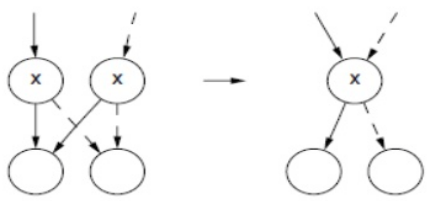
\includegraphics[scale=0.6]{slike/pravilo_spajanja.PNG}
        \caption{Pravilo spajanja}
        \label{fig:reductionRule}
    \end{figure}

    \item Pravilo eliminacije - Ukoliko su visoki i niski naslednici nekog \v{c}vora izomorfni, taj \v{c}vor se uklanja.

    \begin{figure}[H]
        \centering
        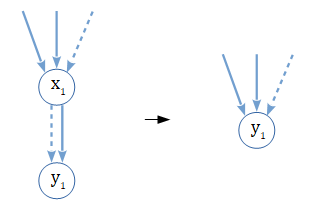
\includegraphics[scale=0.6]{slike/pravilo_eliminacije.PNG}
        \caption{Pravilo eliminacije}
        \label{fig:eliminationRule}
    \end{figure}
\end{itemize}


Mana naivnog pristupa konstrukciji ROBDD je \v{s}to je on uvek eksponencijalne slo\v{z}enosti. Razlog za to je skupo\'c{}a konstrukcije kompletnog binarnog drveta odlu\v{c}ivanja. Pored velike vremenske slo\v{z}enosti, taj proces zauzima i eksponencijalno veliku koli\v{c}inu memorije u odnosu na broj promenljivih u ulaznoj formuli. U nastavku dajemo primer konstrukcije ROBDD (prate\'c{}i naivni pristup koji koristi na\v{s} program, uz prate\'c{}e slike izlaza programa).

\begin{exmp}
    Posmatrajmo funkciju
    $$(x_{1} \vee \overline{x_{2}} \vee \overline{x_{3}}) \wedge (x_{1} \vee \overline{x_{2}} \vee x_{3}) \wedge (x_{1} \vee x_{2} \vee \overline{x_{3}}) \wedge (x_{1} \vee x_{2} \vee x_{3})$$
    Najpre, konstruisa\'c{}emo binarno drvo odlu\v{c}ivanja koje odgovara ovoj funkciji:

    \begin{figure}[H]
        \centering
        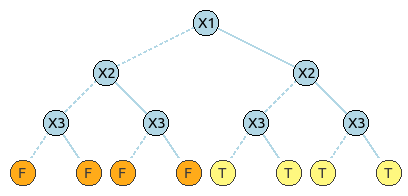
\includegraphics{slike/primer/00.png}
    \end{figure}

    Sada po\v{c}injemo da iteriramo dokle god pravila eliminacije ili spajanja imaju efekta.

    Pravilom spajanja spajamo prva dva podstabla:

    \begin{figure}[H]
        \centering
        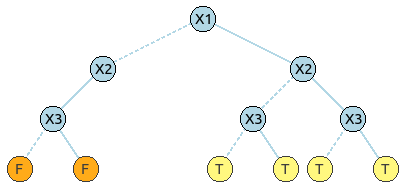
\includegraphics{slike/primer/01.png}
    \end{figure}

    Zatim, takodje pravilom spajanja, spajamo dva \emph{F} \v{c}vora.

    \begin{figure}[H]
        \centering
        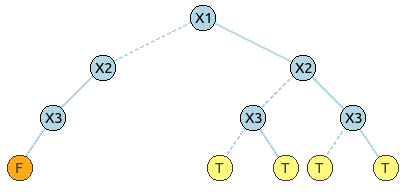
\includegraphics{slike/primer/02.png}
    \end{figure}

    Naredna dva koraka su ekvivalentna prethodnim.

    \begin{figure}[H]
        \centering
        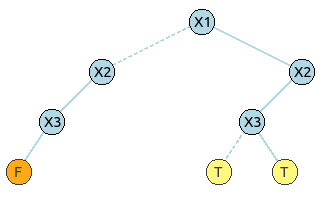
\includegraphics{slike/primer/03.png}
    \end{figure}

    \begin{figure}[H]
        \centering
        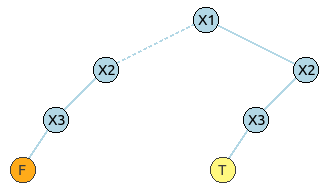
\includegraphics{slike/primer/04.png}
    \end{figure}

    U narednom koraku, pravilom eliminacije, bri\v{s}emo \v{c}vor $x_{2}$.

    \begin{figure}[H]
        \centering
        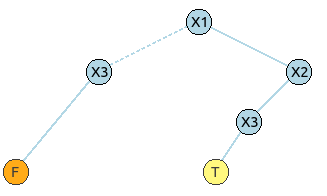
\includegraphics{slike/primer/05.png}
    \end{figure}

    Zatim, pravilom eliminacije, bri\v{s}emo naredni \v{c}vor $x_{3}$.

    \begin{figure}[H]
        \centering
        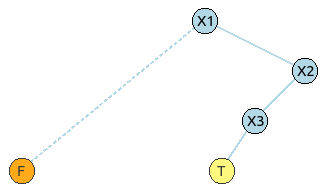
\includegraphics{slike/primer/06.png}
    \end{figure}

    Na ekvivalentan na\v{c}in, uklanjamo preostale \v{c}vorove.

    \begin{figure}[H]
        \centering
        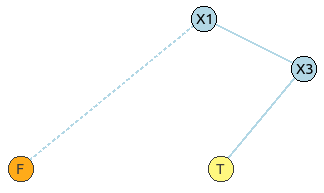
\includegraphics{slike/primer/07.png}
    \end{figure}

    \begin{figure}[H]
        \centering
        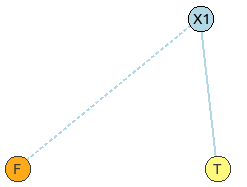
\includegraphics{slike/primer/08.png}
    \end{figure}

    Poslednjim korak predstavlja generisani ROBDD. Kao \v{s}to vidimo, ono je zna\v{c}ajno manje od po\v{c}etnog binarnog stabla odlu\v{c}ivanja. Za izra\v{c}unavanje vrednosti funkcije, dovoljno je ispitati samo vrednost promenljive $x_{1}$.
\end{exmp}


\subsubsection{Optimalna konstrukcija ROBDD}
\label{subsubsec:optimalROBDDConstruction}

Drugi na\v{c}in koji se koristi za konstrukciju ROBDD takodje ima eksponencijalnu slo\v{z}enost. Medjutim, on u praksi daje dobre rezultate. Za razliku od prethodne metode, preska\v{c}e se medjukorak generisanja binarnog uredjenog drveta odlu\v{c}ivanja. Ovo dovodi do smanjenja potrebne memorije za njegovo generisanje, kao i do zna\v{c}ajnog ubrzanja algoritma.

Postupak je rekurzivan: kre\'c{}e se od bulovske funkcije koja se podeli na podfunkcije za koje se najpre generi\v{s}e ROBDD. Naredni korak je spajanje ove dve funkcije u jednu, uz kori\v{s}\'c{}enje pravila eliminacije i spajanja koja su opisana u prethodnoj sekciji.

Naredni primer oslikava efikasnu metodu za generisanje ROBDD.

\begin{exmp}
    Posmatrajmo funkciju
    $$(x_{1} \vee x_{2}) \wedge (\overline{x_{1}} \vee \overline{x_{2}})$$
    Konstruisa\'c{}emo ROBDD u dva koraka, prvo posmatraju\'c{}i $x_{1} \vee x_{2}$ i konstruisati ROBDD za taj deo (rekurzivno), a onda isti postupak primeniti na drugom delu - $\overline{x_{1}} \vee \overline{x_{2}}$. Zatim \v{c}emo spojiti dobijene ROBDD u kona\v{c}ni rezultat.

    Posmatrajmo sada funkciju $x_{1} \vee x_{2}$. Iako ve\'c{} znamo kako izgleda ROBDD za ovu funkciju (pogledati poglavlje \ref{sec:BDD}), kako bismo ispo\v{s}tovali postupak idemo dublje (rekurzivno) i dolazimo do promeljivih $x_{1}$ i $x_{2}$. Pritom, napominjemo da je redosled implicitno izabran tako da $x_{1}$ dolazi pre $x_{2}$ (iako se mo\v{z}e izabrati drugi redosled, sve dok se on svuda po\v{s}tuje). Rezultuju\'c{}i ROBDD su

    \begin{figure}[H]
        \centering
        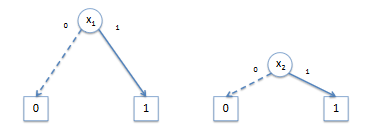
\includegraphics{slike/ROBDD_primer_1.PNG}
    \end{figure}

    Primenjuju\'c{}i bilo koju bulovsku operaciju nad dva ROBDD sa istim redosledom zna\v{c}i krenuti od korena i pratiti paralelne puteve do listova. Kada stignemo do listova, primenjujemo funkciju nad logi\v{c}kom konstantom sadr\v{z}anom u listu kako bismo formirali rezultat za trenutni put. U na\v{s}em primeru, kre\'c{}emo od $x_{1}$ sa levog dijagrama i hipoteti\v{c}kog $x_{1}$ sa desnog dijagrama:

    \begin{figure}[H]
        \centering
        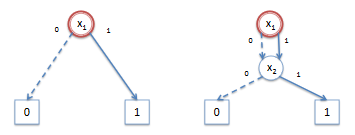
\includegraphics{slike/ROBDD_primer_2.PNG}
    \end{figure}

    Ako pratimo niske grane u oba dijagrama, dolazimo do hipoteti\v{c}kog $x_{2}$ na levom dijagramu i ve\'c{} posstoje\'c{}eg $x_{2}$ na desnom. Napominjemo da je \v{c}vor $x_{2}$ u levom dijagramu samo pomo\'c{} za razumevanje algoritma, u implementaciji se ne bi eksplicitno pravio taj \v{c}vor. Takodje prikazujemo delimi\v{c}no konstruisani rezultuju\'c{}i ROBDD ispod dva ROBDD za promenljive:

    \begin{figure}[H]
        \centering
        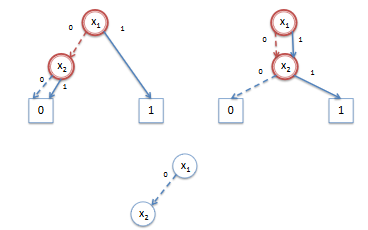
\includegraphics{slike/ROBDD_primer_3.PNG}
    \end{figure}

    S obzirom da niske grane u oba dijagrama vode ka 0, ra\v{c}unamo $0 \vee 0 = 0$ i registrujemo $0$ kao rezultat:

    \begin{figure}[H]
        \centering
        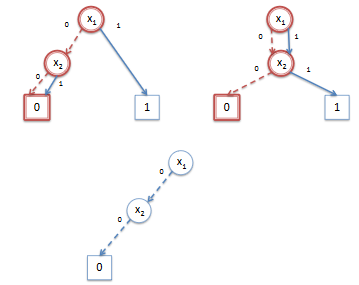
\includegraphics{slike/ROBDD_primer_4.PNG}
    \end{figure}

    Prate\'c{}i visoku granu od $x_{2}$, dolazimo do vrednosti $0$ na levom i $1$ na desnom dijagramu. Primenom funckije dobijamo rezultat $0 \vee 1 = 1$:

    \begin{figure}[H]
        \centering
        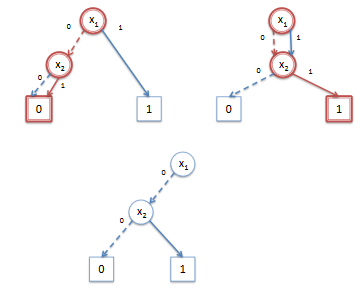
\includegraphics{slike/ROBDD_primer_5.PNG}
    \end{figure}

    Vra\'c{}amo se nazad do $x_{1}$ i razmatramo slu\v{c}aj $x_{1} = 1$ i $x_{2} = 0$. U ovom slu\v{c}aju ra\v{c}unamo $1 \vee 0 = 1$.

    \begin{figure}[H]
        \centering
        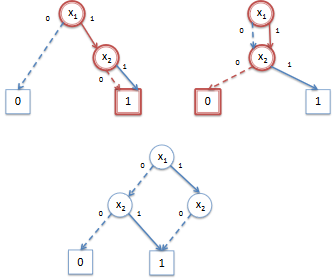
\includegraphics{slike/ROBDD_primer_6.PNG}
    \end{figure}

    Na kraju pratimo visoke grane iz oba $x_{2}$ \v{c}vora i dolazimo do vrednosti $1$:

    \begin{figure}[H]
        \centering
        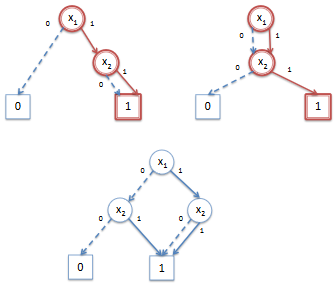
\includegraphics{slike/ROBDD_primer_7.PNG}
    \end{figure}

    Analiziraju\'c{}i rezultat prime\'c{}ujemo da postoje izomorfizmi u konstruisanom dijagramu (pogledati \v{c}vor $x_{2}$ sa desne strane). Stoga, primenjujemo pravilo eliminacije i dobijamo slede\'c{}i rezultat:

    \begin{figure}[H]
        \centering
        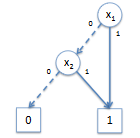
\includegraphics{slike/ROBDD_primer_8.PNG}
    \end{figure}

    ROBDD za funkciju $\overline{x_{1}} \vee \overline{x_{2}}$ se mo\v{z}e dobiti invertovanjem vrednosti u listovima ve\'c{} dobijenog dijagrama. Podsetimo se da smo po\v{c}eli od funkcije $(x_{1} \vee x_{2}) \wedge (\overline{x_{1}} \vee \overline{x_{2}})$ i uspe\v{s}no smo kreirali ROBDD za delove $(x_{1} \vee x_{2})$ i $(\overline{x_{1}} \vee \overline{x_{2}})$, redom:

    \begin{figure}[H]
        \centering
        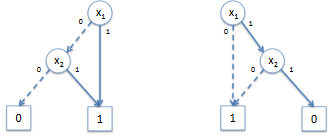
\includegraphics{slike/ROBDD_primer_9.PNG}
    \end{figure}

    Ponavljaju\'c{}i gore opisan postupak za spajanje dijagrama dolazimo do kona\v{c}nog re\v{s}enja:

    \begin{figure}[H]
        \centering
        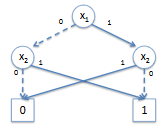
\includegraphics{slike/ROBDD_primer_10.PNG}
    \end{figure}

    Pa\v{z}ljiv \v{c}italac je mo\v{z}da uo\v{c}io sli\v{c}nost funkcije \v{c}iji smo ROBDD konstruisali sa funkcijom $\oplus$ koju smo sreli ranije. Ove dve funkcije su zapravo ekvivalentne. Kako bismo pokazali da se funkcije mogu porediti koriste\'c{}i njihove reprezentacije preko BDD (sve dok su te reprezentacije kanoni\v{c}ne, \v{s}to ROBDD garantuje), mo\v{z}emo se uveriti da va\v{z}i
    $$(x_{1} \vee x_{2}) \wedge (\overline{x_{1}} \vee \overline{x_{2}}) = x_{1} \oplus x_{2}$$
    jer je gore konstruisani dijagram identi\v{c}an dijagramu za funkciju $\oplus$ (videti sliku \ref{fig:BDOrXor}).
\qed
\end{exmp}

\section{Slobodni binarni dijagrami odlu\v{c}ivanja (FBDD)}
\label{sec:FBDD}

Slobodni binarni dijagrami odlu\v{c}ivanja (engl. \emph{Free Binary Decision Diagrams}, u daljem tekstu \emph{FBDD}) koriste \v{S}enonovu dekompoziciju u svakom \v{c}voru (sli\v{c}no kao kod OBDD) ali se du\v{z} razli\v{c}itih putanja mogu koristiti razli\v{c}ita uredjenja. \v{S}tavi\v{s}e, svaka promenljiva se sme testirati samo jednom. Ukoliko se promenljive biraju istim redosledom du\v{z} svih putanja, rezultat je OBDD. Drugim re\v{c}ima, OBDD su specijalan slu\v{c}aj FBDD. Iako nisu u op\v{s}tem slu\v{c}aju kanoni\v{c}ka struktura, uz modifikacije je mogu\'c{}e posti\'c{}i kanoni\v{c}nost. \v{S}tavi\v{s}e, FBDD se efikasno minimizuju i izlistavaju.

Dokazano je  postojanje funkcija koje se mogu efikasno predstaviti pomo\'c{}u FBDD (u polinomijalnom prostoru), dok je za OBDD u najgorem slu\v{c}aju potreban eksponencijalan broj \v{c}vorova. Glavni problem je nepostojanje efikasne heuristike za odabir redosleda promenljivih. Iako postoji dosta pristupa za re\v{s}avanje pomenutog problema [4, 5, 6], nije pronadjeno zna\v{c}ajno br\v{z}e unapredjenje u odnosu na OBDD.

SAT re\v{s}ava\v{c}i se mogu koristiti za konstrukciju i minimizaciju FBDD. SAT re\v{s}ava\v{c}i se mogu shvatiti kao pretra\v{z}iva\v{c}i binarnog stabla odlu\v{c}ivanja za datu funkciju. U op\v{s}tem slu\v{c}aju, uz fiksni izbor odabira promenljivih u implementaciji SAT re\v{s}ava\v{c}a, drvo koje SAT re\v{s}ava\v{c} pretra\v{z}uje je zapravo OBDD. U slu\v{c}aju nedeterministi\v{c}kog izbora promenljivih, to drvo je FBDD.

U nastavku se podrazumeva da je \v{c}italac upoznat sa terminima iskazne logike. Prvo \'c{}emo, uz kori\v{s}\'c{}enje SAT re\v{s}ava\v{c}a, opisati proces konstrukcije FBDD (deo \ref{subsec:FBDDConstructionViaSAT}), a zatim proces minimizacije FBDD (deo \ref{subsec:?}).


\section{Konstrukcija FBDD uz pomo\'c{} SAT re\v{s}ava\v{c}a}
\label{subsec:FBDDConstructionViaSAT}

SAT re\v{s}ava\v{c}i pronalaze valuaciju $v$ takvu da je $f(v) = 1$ za datu funkciju $f$, ili pokazuju nepostojanje takvog $v$. Tokom procesa pretrage valuacija, prave se razni izbori i implikacije. Posmatranjem procesa pronala\v{z}enja pomenute valuacije mo\v{z}emo definisati osnovne osobine koje proces konstrukcije FBDD mora da ispunjava:

\begin{obsn}
    Neka je data bulovska funkcija $f : \mathbb{B}^{n} \rightarrow \mathbb{B}$  u KNF normalnoj formi. Tada va\v{z}i:
    \begin{itemize}
        \item Svaka valuacija koja zadovoljava $f$ odgovara putu koji vodi ka vrednosti $1$ u FBDD koji predstavlja $f$.
        \item Svaka konfliktna valuacija odgovara putu koji vodi ka vrednosti $0$ u FBDD koji predstavlja $f$.
        \item Svaka implikacija $x_{i} = b$, gde je $x \in f, b \in \mathbb{B}$ odgovara putu koji vodi ka vrednosti $0$ u FBDD koji predstavlja $f$. Ovaj put se moze konstruisati koriste\'c{}i trenutnu parcijalnu valuaciju $v$ uz $x_{i} = \overline{b}$.
    \end{itemize}
\end{obsn}

% TODO PRIMER?

\section{Binarni dijagrami odlu\v{c}ivanja sa potisnutim nulama (ZSBDD)}
\label{sec:ZSBDD}

Lorem ipsum dolor sit amet, consectetur adipisicing elit, sed do eiusmod tempor incididunt ut labore et dolore magna aliqua. Ut enim ad minim veniam, quis nostrud exercitation ullamco laboris nisi ut aliquip ex ea commodo consequat. Duis aute irure dolor in reprehenderit in voluptate velit esse cillum dolore eu fugiat nulla pariatur. Excepteur sint occaecat cupidatat non proident, sunt in culpa qui officia deserunt mollit anim id est laborum.

\section{Zaklju\v{c}ak}
\label{sec:Zakljucak}

U ovom radu su prikazane osnovne strukture podataka za predstavljanje bulovskih funkcija. BDD predstavljaju mo\'c{}an alat za rad sa bulovskim funkcijama, i uz pobolj\v{s}anje algoritama i pronalascima optimalnijih varijanti BDD, mogu\'c{}e je predstaviti konstruisati BDD veoma komplikovanih funkcija u prihvatljivom vremenu. Takodje, uz pobolj\v{s}anje SAT re\v{s}ava\v{c}a koji danas mogu da za manje od sekunde provere zadovoljivost formula sa stotinama hiljada klauza, FBDD pomeraju granice broja ulaznih argumenata u funkciju. Uz ovaj rad prila\v{z}emo i implementaciju BDT i redukciju BDT u ROBDD u programskom jeziku C++.


\addcontentsline{toc}{section}{Literatura}
\bibliographystyle{plain}
\bibliography{literatura}

\newpage

%\begin{appendices}
%\input{delovi/???}
%\end{appendices}

\end{document}
